\subsection{Sensorik}
\label{Sensorik_sec}
Die Aufgabe der verwendeten Sensorik liegt darin die Werte für $\varphi$, und $\dot{\varphi}$ zu bestimmen. Hierfür wurden zwei MPU6050 IC's verwendet. Diese verfügen jeweils über einen Beschleunigungssensor und Gyroskop, welche Werte für drei Achsen ausgeben. Der Tiefpass der Sensoren wird auf eine Grenzfrequenz von $44Hz$ eingestellt, da hier einerseits eine erste Glättung der Daten erfolgt, andererseits aber keine zu große Verzögerung ergibt, welche sich wiederum negativ auf die Regelung auswirken könnte. Die Position und Ausrichtung der Sensoren ist in \ref{Position_Sensoren_pic} dargestellt.

\begin{figure}[h]
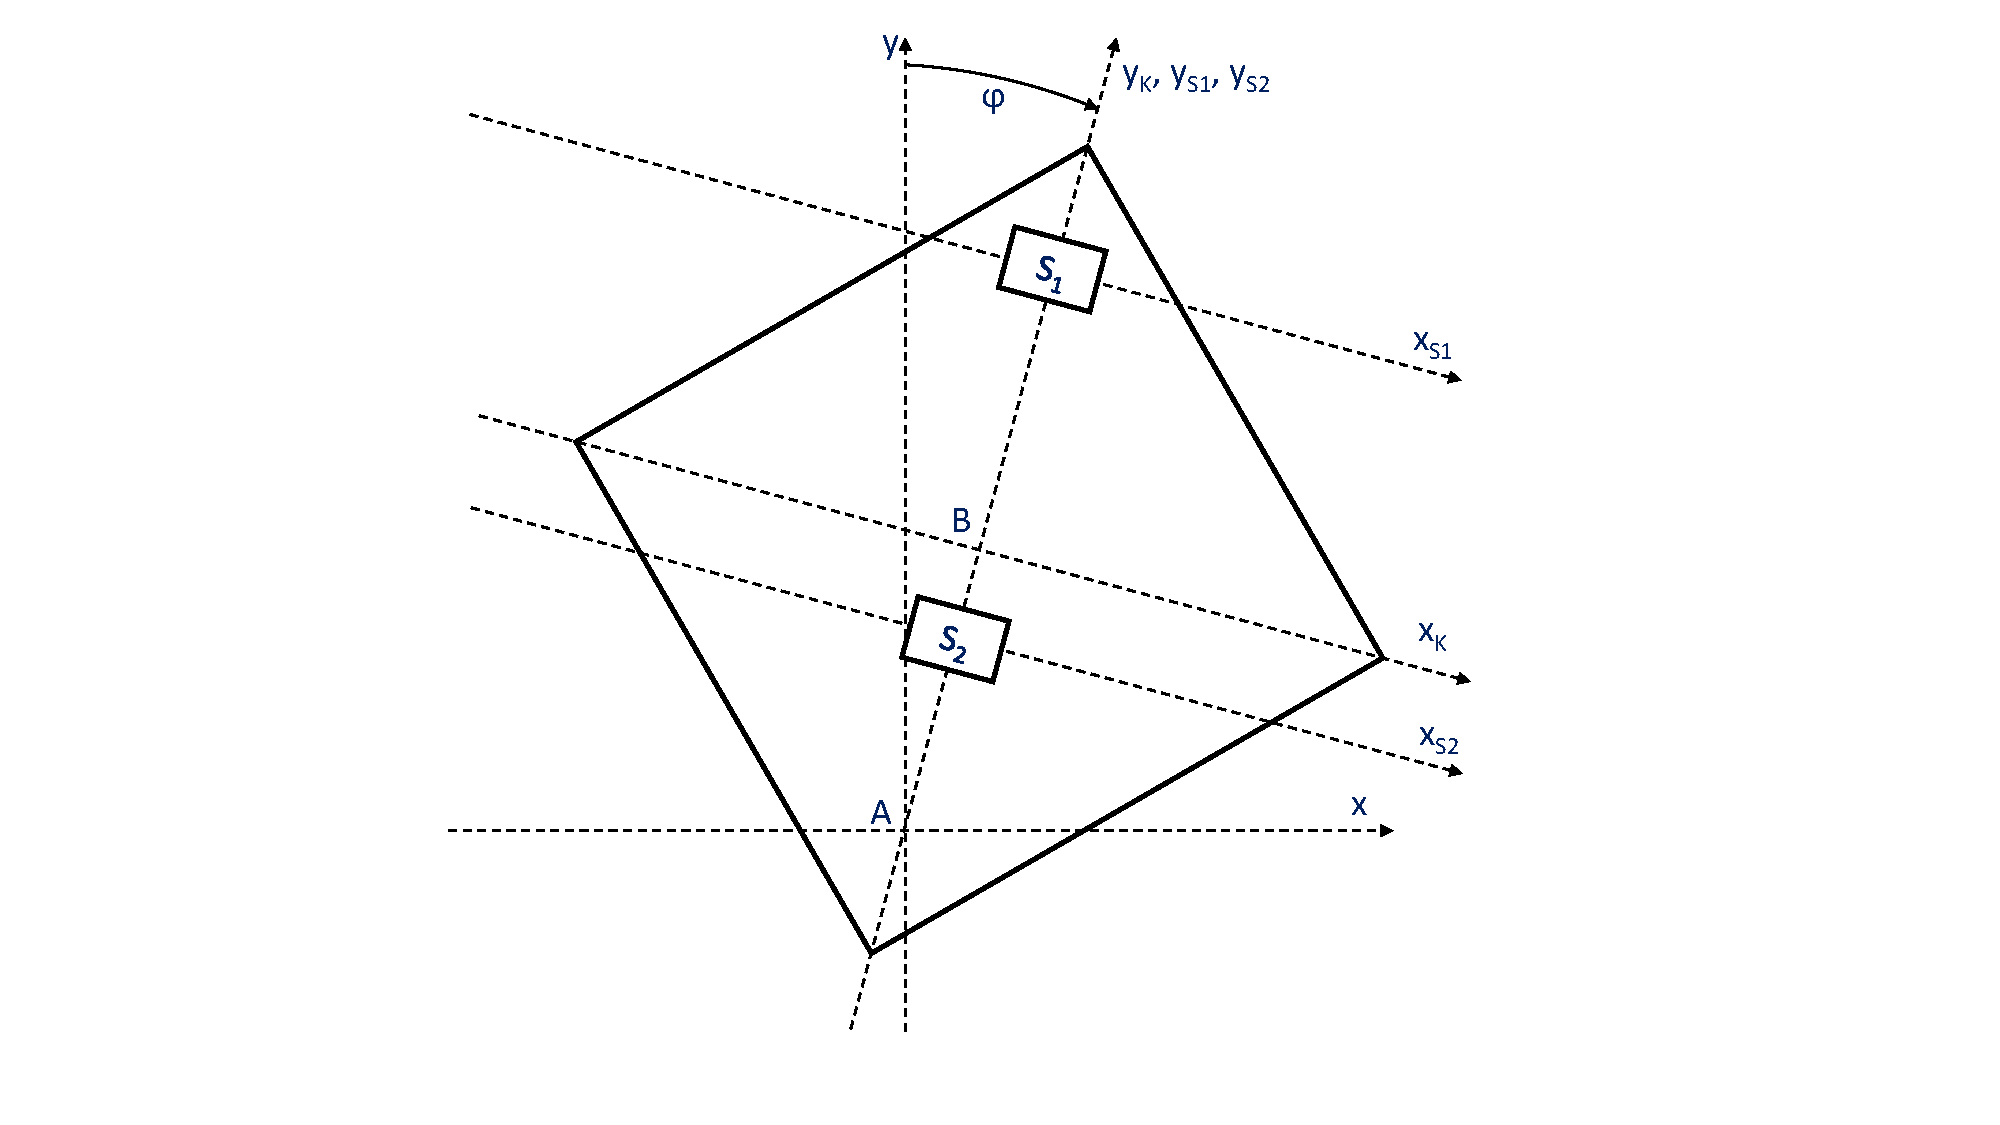
\includegraphics[width=\linewidth]{SensorZeichnung1D}
\caption{Position der Sensoren, Quelle: eigene Darstellung}

\label{Position_Sensoren_pic}
\end{figure}

\subsubsection{Winkelschätzung}
Die Sensoren sind nicht in der Lage Wege bzw. Winkel zu messen. Somit muss der Winkel $\varphi$ berechnet werden. Die gemessenen Beschleunigungen setzten sich aus einem statischen Anteil, welcher von $\varphi$ abhängt, und einem dynamischen Anteil, welcher von $\dot{\varphi}$ bzw. $\ddot{\varphi}$ abhängt, zusammen.

\begin{equation}
\ddot{S}_i = 
\begin{pmatrix}
\ddot{x}_i \\ \ddot{y}_i \\ \ddot{z}_i
\end{pmatrix} =
\begin{pmatrix}
r_{Si} \cdot \ddot{\varphi} + sin(\varphi) \cdot g \\
- r_{Si} \cdot \dot{\varphi}^2 - cos(\varphi) \cdot g \\
0
\end{pmatrix}
\hspace{35pt}
i \in [1;2]
\end{equation}

Da die dynamischen Anteile zusätzlich von dem Abstand $r_{Si}$ abhängen, kann die geometrische Anordnung der beiden Sensoren genutzt werden um das Verhältnis der beiden Anteile zu berechnen. Somit kann der aktuelle Wert von $\varphi$ nach \cite{Cubli1D} wie folgt berechnen.
\begin{equation}
\alpha = \frac{r_{S1}}{r_{S2}}
\end{equation}

\begin{equation}
\ddot{x}_1 - \alpha \cdot \ddot{x}_2 = 
g(1 - \alpha)sin(\varphi)
\end{equation}
\begin{equation}
\ddot{y}_1 - \alpha \cdot \ddot{y}_2 = 
-g(1- \alpha)cos(\varphi)
\end{equation}

\begin{equation}
\frac{\ddot{x}_1 - \alpha \cdot \ddot{x}_2}{\ddot{y}_1 - \alpha \cdot \ddot{y}_2} = -tan(\varphi)
\end{equation}

Nach dem selben Prinzip kann auch die Winkelbeschleunigung $\ddot{\varphi}$ berechnet werden.
\begin{equation}
\ddot{x}_1 - \ddot{x}_2 = [r_{S1} \cdot \ddot{\varphi} + sin(\varphi) \cdot g] - [r_{S2} \cdot \ddot{\varphi} + sin(\varphi) \cdot g] = (r_{S1} - r_{S2}) \cdot \ddot{\varphi}
\end{equation}
\begin{equation}
\ddot{\varphi} = \frac{\ddot{x}_1 - \ddot{x}_2}{r_{S1} - r_{S2}}
\end{equation}

\subsubsection{Kalibrierung und Justierung}
Die Sensoren geben die Beschleunigungs- und Geschwindigkeitswerte als 16 Bit Werte im Zweierkomplement aus. Diese Rohwerte müssen in die mit Hilfe eines Ausgleichspolynoms in die jeweilige SI-Einheit umgerechnet werden. 

\subsubsubsection{Umrechnung der Beschleunigungswerte}
Um das Polynom zur Umrechnung der Beschleunigungswerte zu ermitteln werden sieben Messungen in den fixen Ausfallpositionen $\phi \in [-45, -30, -15, 0, 15, 30, 45]$ durchgeführt. Pro Position werden $m = 10000$ Messwerte aufgenommen. Da in der Ruhelage die Beschleunigung lediglich von dem aktuellen Ausfallwinkel abhängt ist der Sollwert für jede Position bekannt. Somit kann ein Polynom erster Ordnung approximiert werden um Mittelwerte der sieben Positionen in die entsprechenden Beschleunigungswerte umzurechnen.

\begin{table}[h]
\centering
\begin{tabular}{lcllcl}
$\ddot{x}_n$ &$\equiv$& X-Beschleunigung Sensor n &
$\ddot{x}^R_n$ &$\equiv$& X-Rohwert Sensor n \\
$\ddot{y}_n$ &$\equiv$& Y-Beschleunigung Sensor n &
$\ddot{y}^R_n$ &$\equiv$& Y-Rohwert Sensor n
\end{tabular}
\end{table}

\vspace*{-\baselineskip}
\begin{equation}
\ddot{x}_n = p^1_{x_n} \cdot \ddot{x}^R_n + p^2_{x_n} \hspace{35pt} \vert \hspace{3pt} n \in \{1, 2\}
\end{equation}
\begin{equation}
\ddot{y}_n = p^1_{y_n} \cdot \ddot{y}^R_n + p^2_{y_n} \hspace{35pt} \vert \hspace{3pt} n \in \{1, 2\}
\end{equation}
\vspace*{-\baselineskip}
\begin{table}[h]
\centering
\begin{tabular}{lcllcl}
$p^1_{x_1}$ &$=$& $-5.992 \cdot 10^{-4}$ & $p^2_{x_1}$ &$=$& $0.3328$ \\
$p^1_{x_2}$ &$=$& $-6.003 \cdot 10^{-4}$ & $p^2_{x_2}$ &$=$& $0.4138$ \\
$p^1_{y_1}$ &$=$& $-6.127 \cdot 10^{-4}$ & $p^2_{y_1}$ &$=$& $0.1186$ \\
$p^1_{y_2}$ &$=$& $-6.81 \cdot 10^{-4}$ & $p^2_{y_2}$ &$=$& $0.1143$ \\
\end{tabular}
\end{table}

\vspace*{-\baselineskip}
\begin{figure}[h]
	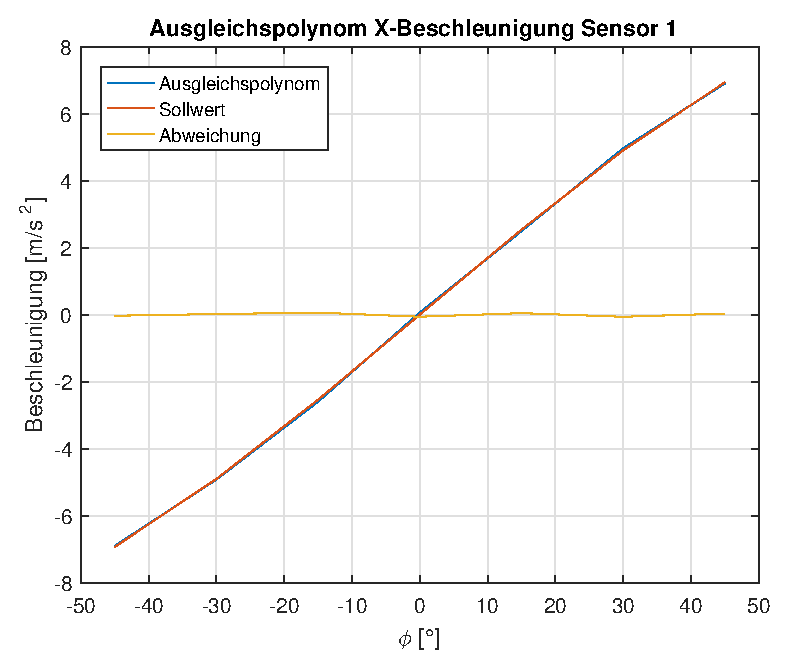
\includegraphics[width=0.5\linewidth]{img/X1__dd___fitted.eps}
	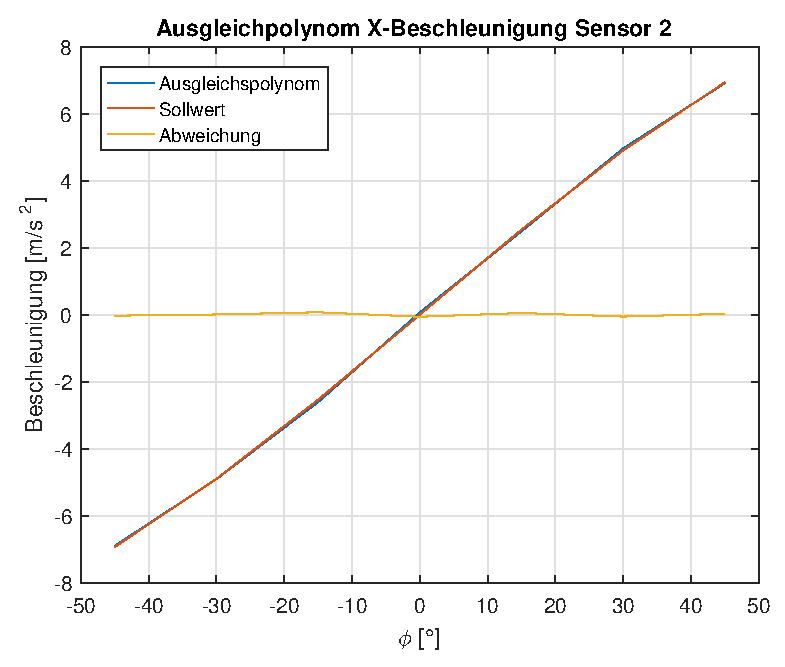
\includegraphics[width=0.5\linewidth]{img/X2__dd___fitted.eps}
\end{figure}

\vspace*{-\baselineskip}
\begin{figure}[h!]
	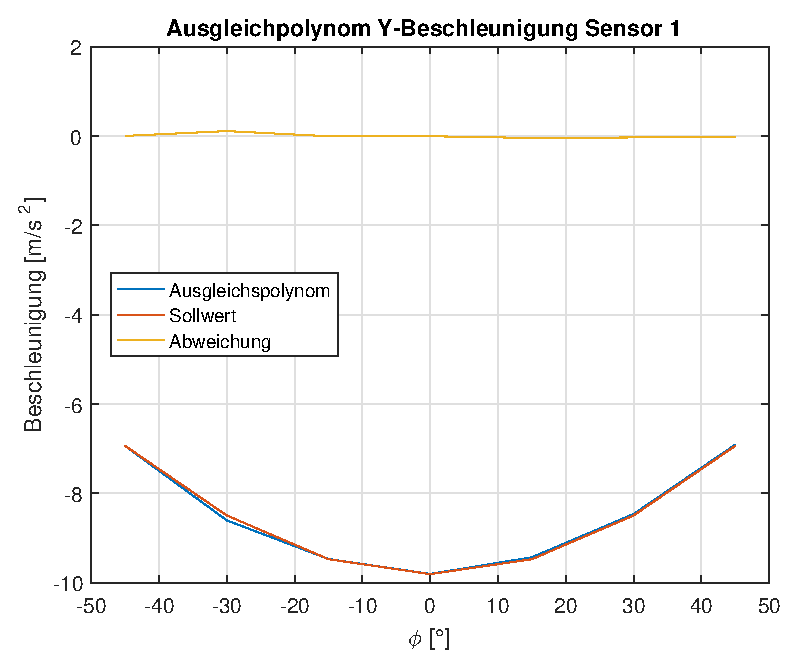
\includegraphics[width=0.5\linewidth]{img/Y1__dd___fitted.eps}
	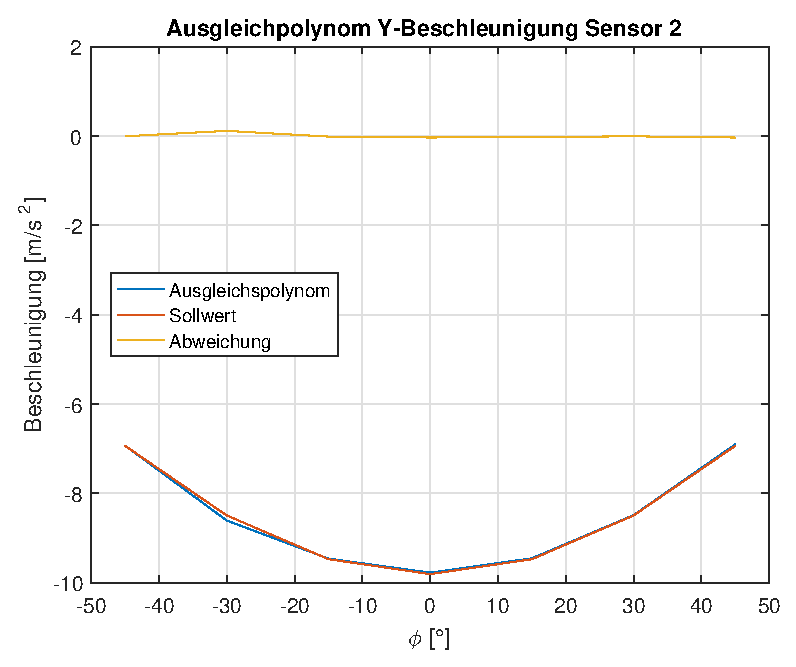
\includegraphics[width=0.5\linewidth]{img/Y2__dd___fitted.eps}
\end{figure}

\subsubsubsection{Umrechnung der Winkelgeschwindigkeiten}
Um die Rohwerte der Gyroskope in Winkelgeschwindigkeiten umzurechnen wird die Würfelseite fixiert und die Winkelgeschwindigkeitswerte der beiden Sensoren aufgenommen. Hierbei werden jeweils $m = 1000$ Werte aufgenommen. Da der Sollwert $\dot{\varphi} = 0 \frac{m}{s}$ bekannt ist kann die systematische Messabweichung der Sensoren über den Mittelwert bestimmt werden. Der proportionale Umrechnungsfaktor von Rohdaten zu Winkelgeschwindigkeiten wird dem Datenblatt des Herstellers entnommen.
\begin{figure}[h]
	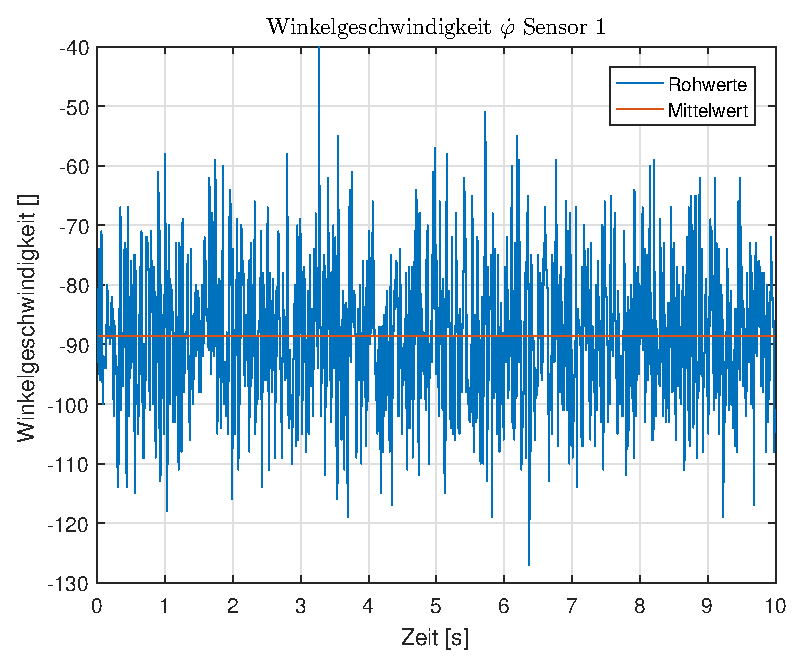
\includegraphics[width=0.5\linewidth]{img/phi1__d.eps}
	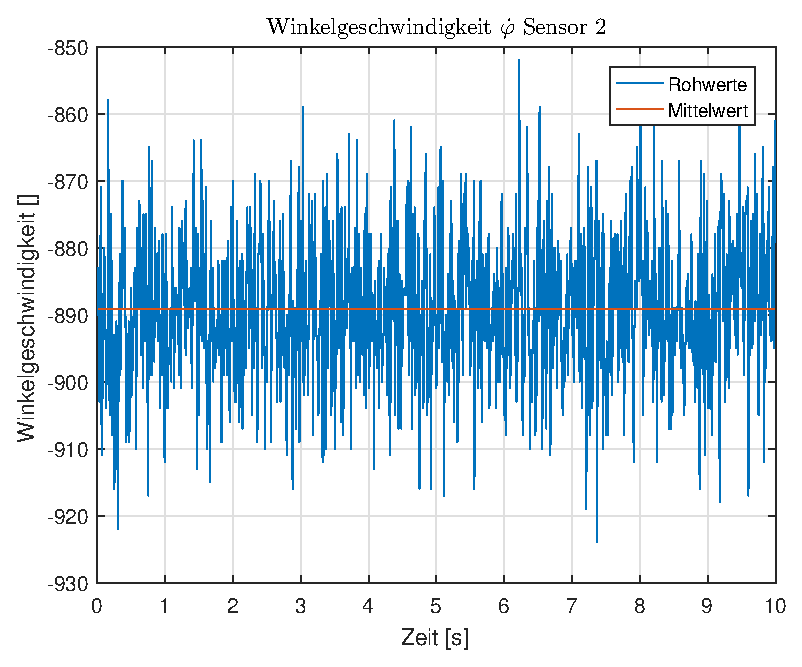
\includegraphics[width=0.5\linewidth]{img/phi2__d.eps}
\end{figure}
\vspace*{-\baselineskip}
\begin{table}[h]
\centering
\begin{tabular}{lcllcl}
$\dot{\varphi}_n$ & $\equiv$ & $\varphi$-Geschwindigkeit Sensor n & $\dot{\varphi}^R_n$ & $\equiv$ $\dot{\varphi}$-Rohwert Sensor n
\end{tabular}
\end{table}
\vspace*{-\baselineskip}
\begin{equation}
\dot{\varphi}_n = p^1_{\dot{\varphi}^R_n}  \cdot (\dot{\varphi}_n + p^2_{\dot{\varphi}_n})
\end{equation}
\vspace*{-\baselineskip}
\begin{table}[h]
\centering
\begin{tabular}{lcllcl}
$p^1_{\varphi_1}$ &$=$& $-1.3265 \cdot 10^{-4}$ & $p^2_{\varphi_1}$ &$=$& $441.3160$ \\
$p^1_{\varphi_2}$ &$=$& $-1.3265 \cdot 10^{-4}$ & $p^2_{\varphi_2}$ &$=$& $76.5140$ \\
\end{tabular}
\end{table}
\vspace*{-\baselineskip}
\subsubsection{Auswertung der Radgeschwindigkeit $\dot{\psi}$}
Der Motortreiber liefert ein analoges Spannungssignal, welches die aktuelle Motorgeschwindigkeit wiedergibt. Um die ADC-Werte in SI-Einheiten umzurechnen wird ein Polynom erster Ordnung benötigt. Hierfür werden mit Hilfe der ESCON-Studio konstante Motorgeschwindigkeiten ($\dot{\psi} \in \{ -3000, -2000,$  $-1000, 0, 1000, 2000, 3000 \} [rpm] $) gefahren und pro Durchlauf $m=500$ ADC-Werte aufgenommen. Über die Mittelwerte der Messungen und die vorgegebenen Radgeschwindigkeiten wird anschließend ein Polynom erster Ordnung approximiert.
\begin{table}[h!]
\centering
\begin{tabular}{lcllcl}
$\dot{\psi}$ & $\equiv$ & Geschwindigkeit der Schwungmasse & $\dot{\psi}_{ADC}$ & $\equiv$ & ADC-Wert
\end{tabular}
\end{table}
\vspace*{-\baselineskip}
\begin{equation}
\dot{\psi} = -0.5092 \cdot \dot{\psi}_{ADC} + 1050
\end{equation}
\vspace*{-\baselineskip}
\begin{figure}[h!]
\centering
	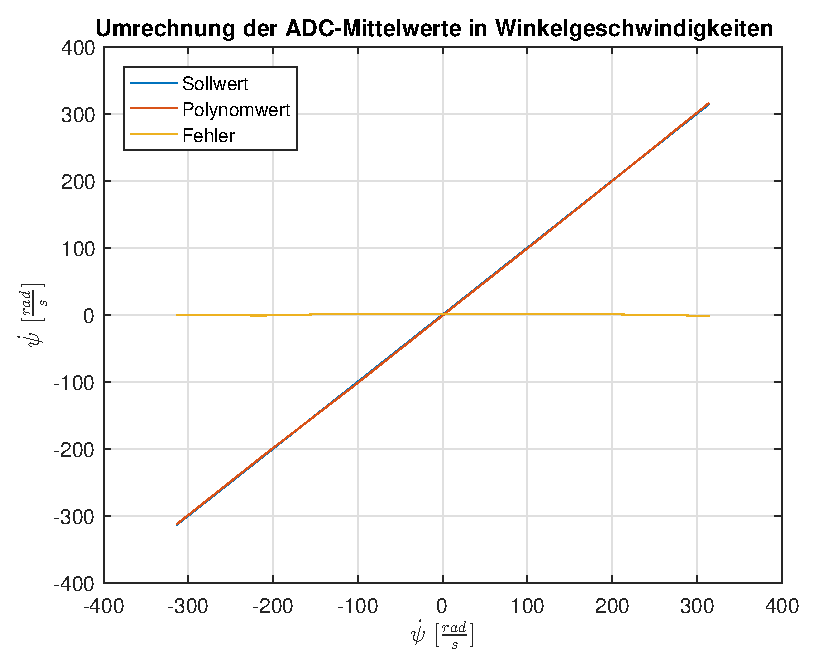
\includegraphics[width=0.5\linewidth]{img/ADC_mittelwert_polynom.eps}
\end{figure}
